\documentclass[tikz]{standalone}
\usepackage{tikz}
\usepackage{alphalph}
\usetikzlibrary{positioning, graphs}
\usetikzlibrary{graphs.standard}
\begin{document}
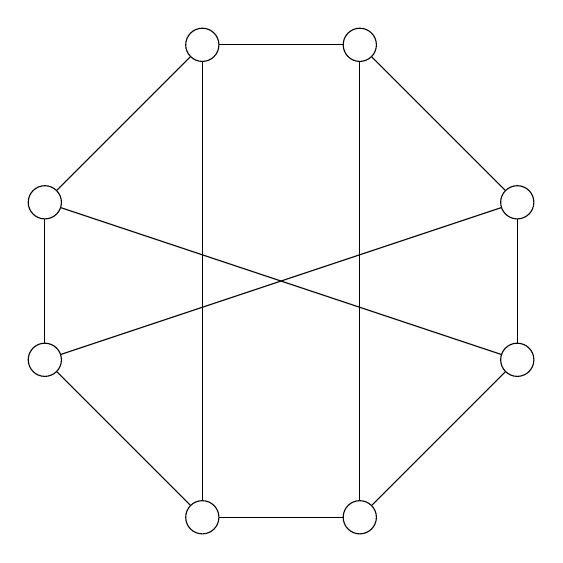
\begin{tikzpicture}
\begin{scope}
		[vertex/.style={draw,circle,inner sep = 0em, minimum size = 1.2em},
		 edgelabel/.style = {fill = white, inner sep = 0.2em, font=\small}]
		\node[vertex] (a) at (2, 6) {};
		\node[vertex] (b) at (4, 6) {};
		\node[vertex] (c) at (0, 4) {};
		\node[vertex] (d) at (6, 4) {};
		\node[vertex] (e) at (0, 2) {};
		\node[vertex] (f) at (6, 2) {};
		\node[vertex] (g) at (2, 0) {};
		\node[vertex] (h) at (4, 0) {};
		
        \draw[-] (a) to (b);
        \draw[-] (a) to (c);
        \draw[-] (a) to (g);
        \draw[-] (b) to (d);
        \draw[-] (b) to (h);
        \draw[-] (c) to (e);
        \draw[-] (c) to (f);
        \draw[-] (d) to (e);
        \draw[-] (d) to (f);
        \draw[-] (e) to (g);
        \draw[-] (f) to (h);
        \draw[-] (g) to (h);

		
\end{scope}
\end{tikzpicture}
\end{document}